\section{Introduction}

Computer operations specify the identities of the particular registers and memory addresses they read and act on.
Computer programs, composed of these individual operations, often additionally specify higher-level elements such as flow markers and functions.
We will refer to computational elements that are specified among by a computer program as operands.
The term queries will describe sites in the computer program where a operand is specified.

As instances of computer programs, genetic programs must also specify computational elements on which to act.
Several approaches to addressing this problem have arisen.

Operands may be implicitly specified according to the position of a query in a genetic program.
Tree-based GP, which traditionally represent programs as a rooted binary trees of operations, exemplify this approach.
An operation's inputs are simply the outputs of its child nodes.
%Lones and Tyrell commmentary: mutational operator disaster
%potentially restricts possible topologies?

A second possibility is to enumerate all possible operands, assign each a operand unique identifier, and then encode an identifier for each query.
However, this approach doesn't effectively support the addition or removal of operands.
%* too many options first = miniscule probability of connecting
%* too few options next

Tag-matching constitutes a third possible solution.
This approach encodes a tag for each query and for each available operand.
Then, operands are specified for each query through a tag-matching process where the query tag is compared to all available operand tags and the best-matching operand is selected.
Queries may be dereferenced prior to program evaluation (e.g., static) or during program evaluation (e.g., dynamic), potentially allowing for program state to influence which operands are specified by queries.
This third idea is similar to the second except that it allows for the number of operands to change without the need for a complicated and potentially arbitrary mutation operator to update invalidated queries.

%Duplication and deletion of genes (e.g., modules) is important in evolutionary biology in the evolution of complex features (TODO cite).
%Genetic program representations that accommodate such events might help GP benefit from these events .
What are the benefits of tags/tag-based referencing?

\begin{itemize}
  \item Hypothesis: Inexactness allowed by tag-based referencing makes these references
        more robust to minor genetic perturbations, smoothing the genotype-phenotype
        mapping relative to more traditional memory-indexing techniques (pulled from
        2019 Tag-access memory abstract).
  \item We don't need to know/lock-in the architecture of what our tags are referencing.
        If a referent (e.g., module) is deleted, it doesn't invalidate any of the
        in-program references (e.g., module calls). The same is true for creating
        a new referent. For example, using tags to reference program modules allows
        you to mutate the number of modules in the program without (necessarily)
        breaking existing references.
  \item Hypothesis: Tag-based referencing should help to enable the duplication/
        deletion of referents (e.g., modules), which should improve capacity for
        complexity to evolve (i.e., duplication is often cited as important in the
        evolution of complex features).
\end{itemize}

A fourth, intriguing approach closely related to tag-matching was developed by Lones and Tyrell in their enzyme genetic programming system, where program sub-modules are labeled according to a functional profile derived from the component's composition and interface \citep{lones2002biomimetic}.

The notion of tags is not unique to genetic programming.
Other digital evolution subdomains have also made effective use of tag-matching techniques (cite... Markov brains? neuroevolution?).

Spector et al. pioneered the use of tag-matching schemes in genetic programming.
In \citep{spector2011tag}, Spector et al. use an integer-based tagging and tag-matching to retrieve data items from PushGP stacks, including code modules (TODO @amlalejini is this right?).

In existing work, the event-driven genetic programming representation SignalGP has used a hamming-distance-based tag-matching scheme to activate program modules in response to tagged events.
In \citep{lalejini2018evolving}, Lalejini and Ofria demonstrate the event-driven paradigm realized with tag-matching yields better-performing evolved solutions to an environmental state tracking problem and a distributed leader-election problem.
In \citep{lalejini2019}, Lalejini and Ofria investigate the consequences of applying a minimum match-quality cutoff threshold.
Requiring exact or near-exact matches cripples the rate of adaptive evolution against the environmental state tracking problem, ostensibly because the probabilities of establishing event-module connections through mutation becomes miniscule.
On the other hand, enforcing only a low match-quality quality cutoff threshold reduces the quality of evolved solutions in the presence of additional irrelevant environmental cues.

Spector et al. use an integer-based tagging system, while Lalejini and Ofria use a hamming-distance based tagging system.
In \citep{downing2015intelligence}, Downing proposes a tag-matching metric based on the lengths of matching and mismatching streaks between two bitstrings but does not demonstrate it in an evolving system.
(We formally characterize these tag-matching systems in our Methods section.)

Although these tag-matching systems all suffice to match queries and operands, they may vary meaningfully with respect to the graph structures of query-operand matches they can represent and do statically tend to represent.
Here, we set out to test different properties of tag-matching systems with respect to geometrical constraint, mutational outcomes, and evolutionary dynamics.

%Metric dimensionality constrains the possible relative orderings of matches.
%A one-dimensional metric can represent all possible query-to-single-operand lookups.
%However, it can not represent all possible query-to-multiple-operand lookups
%This, of course, is relevant to a system where a query matches with multiple operands.
%In a dynamically matched query-to-single-operand system, however, this can be relevant to the resulting connectivity under runtime silencing or upregulation of modules.
%However, even in a static system, this can be relevant to resulting connectivity under deletion of an operand.

%Figure \ref{fig:1d-2d-single-double} provides an example of a set of two-match orderings that a one-dimensional metric, like the integer metric, cannot represent.
%\begin{figure}
\begin{center}

\begin{subfigure}[b]{\columnwidth}
\centering
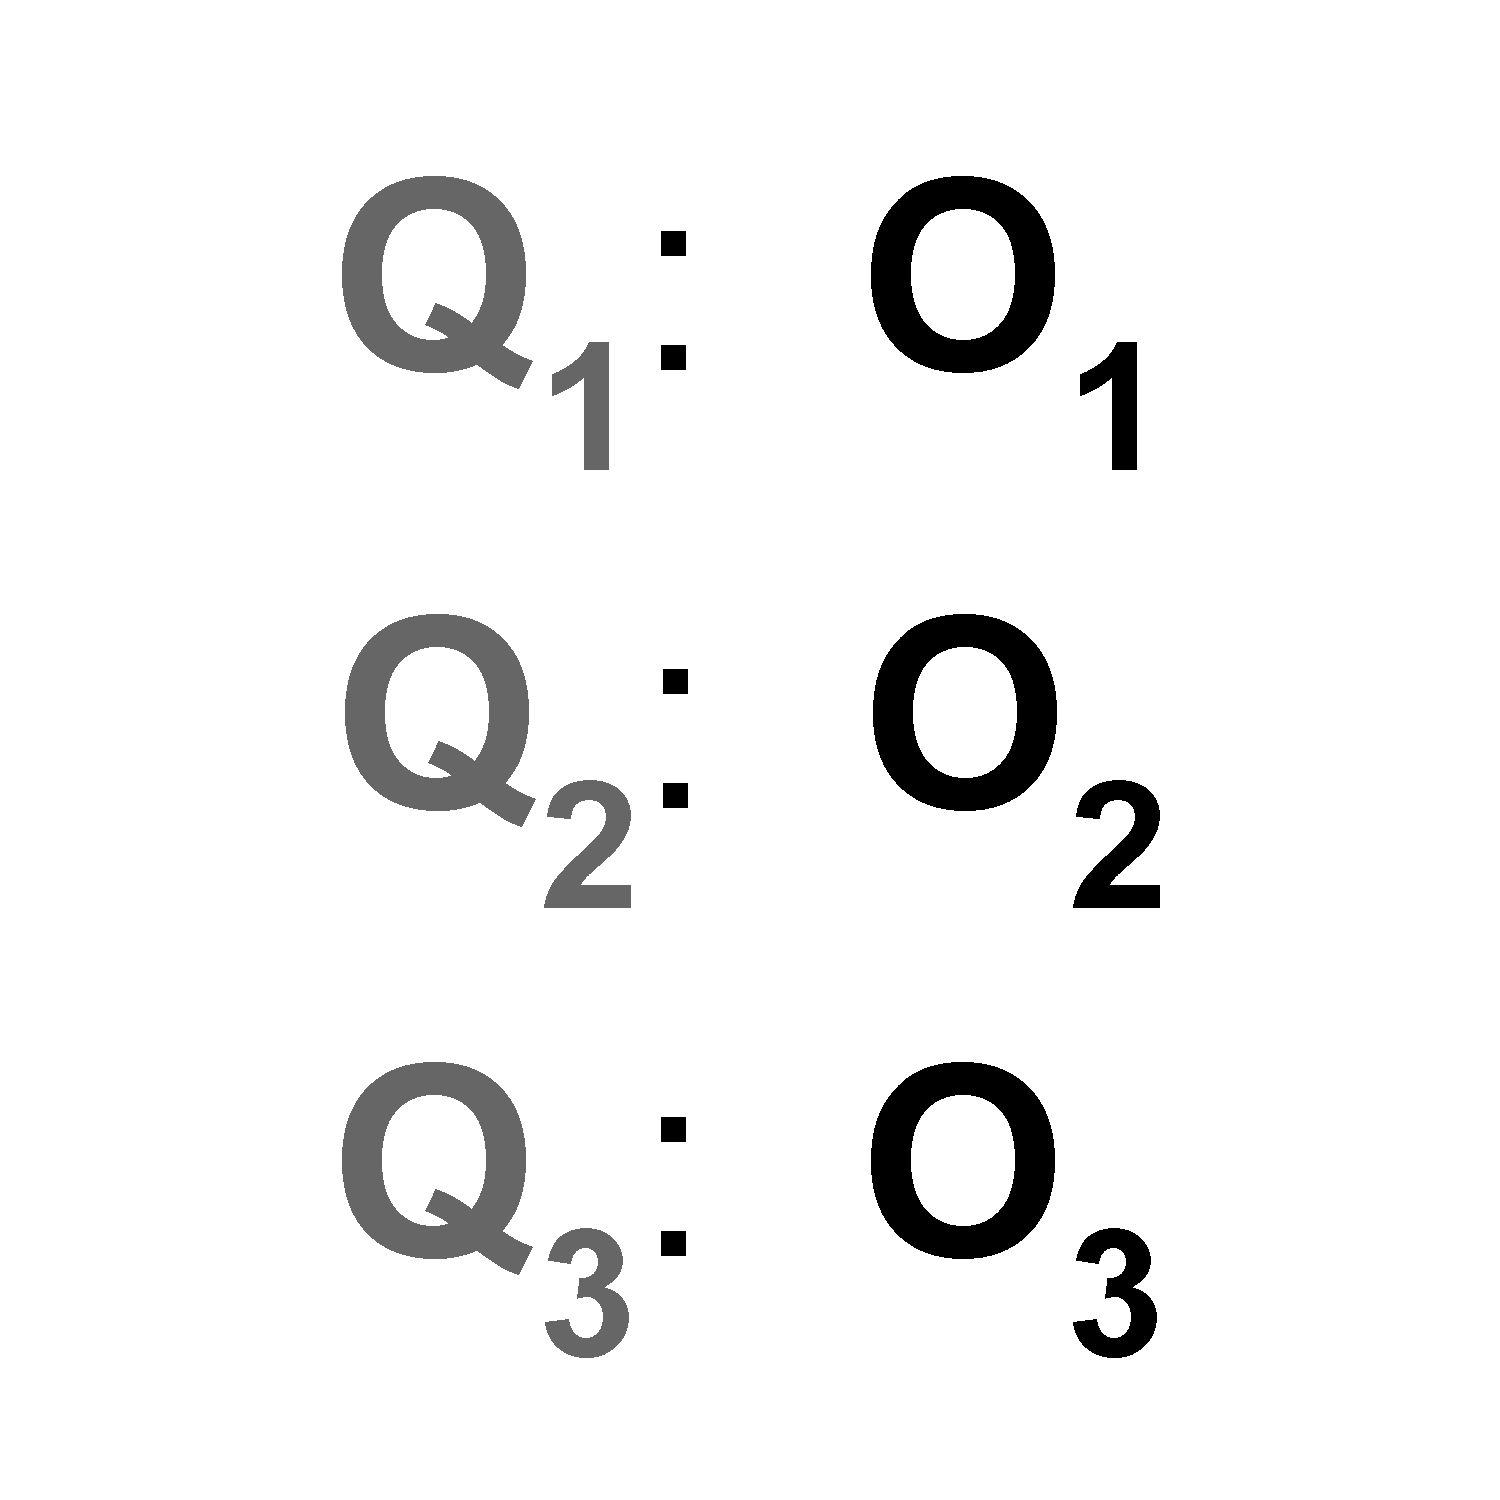
\includegraphics[width=0.33\columnwidth]{{{1d-2d-single-double/single}}}%
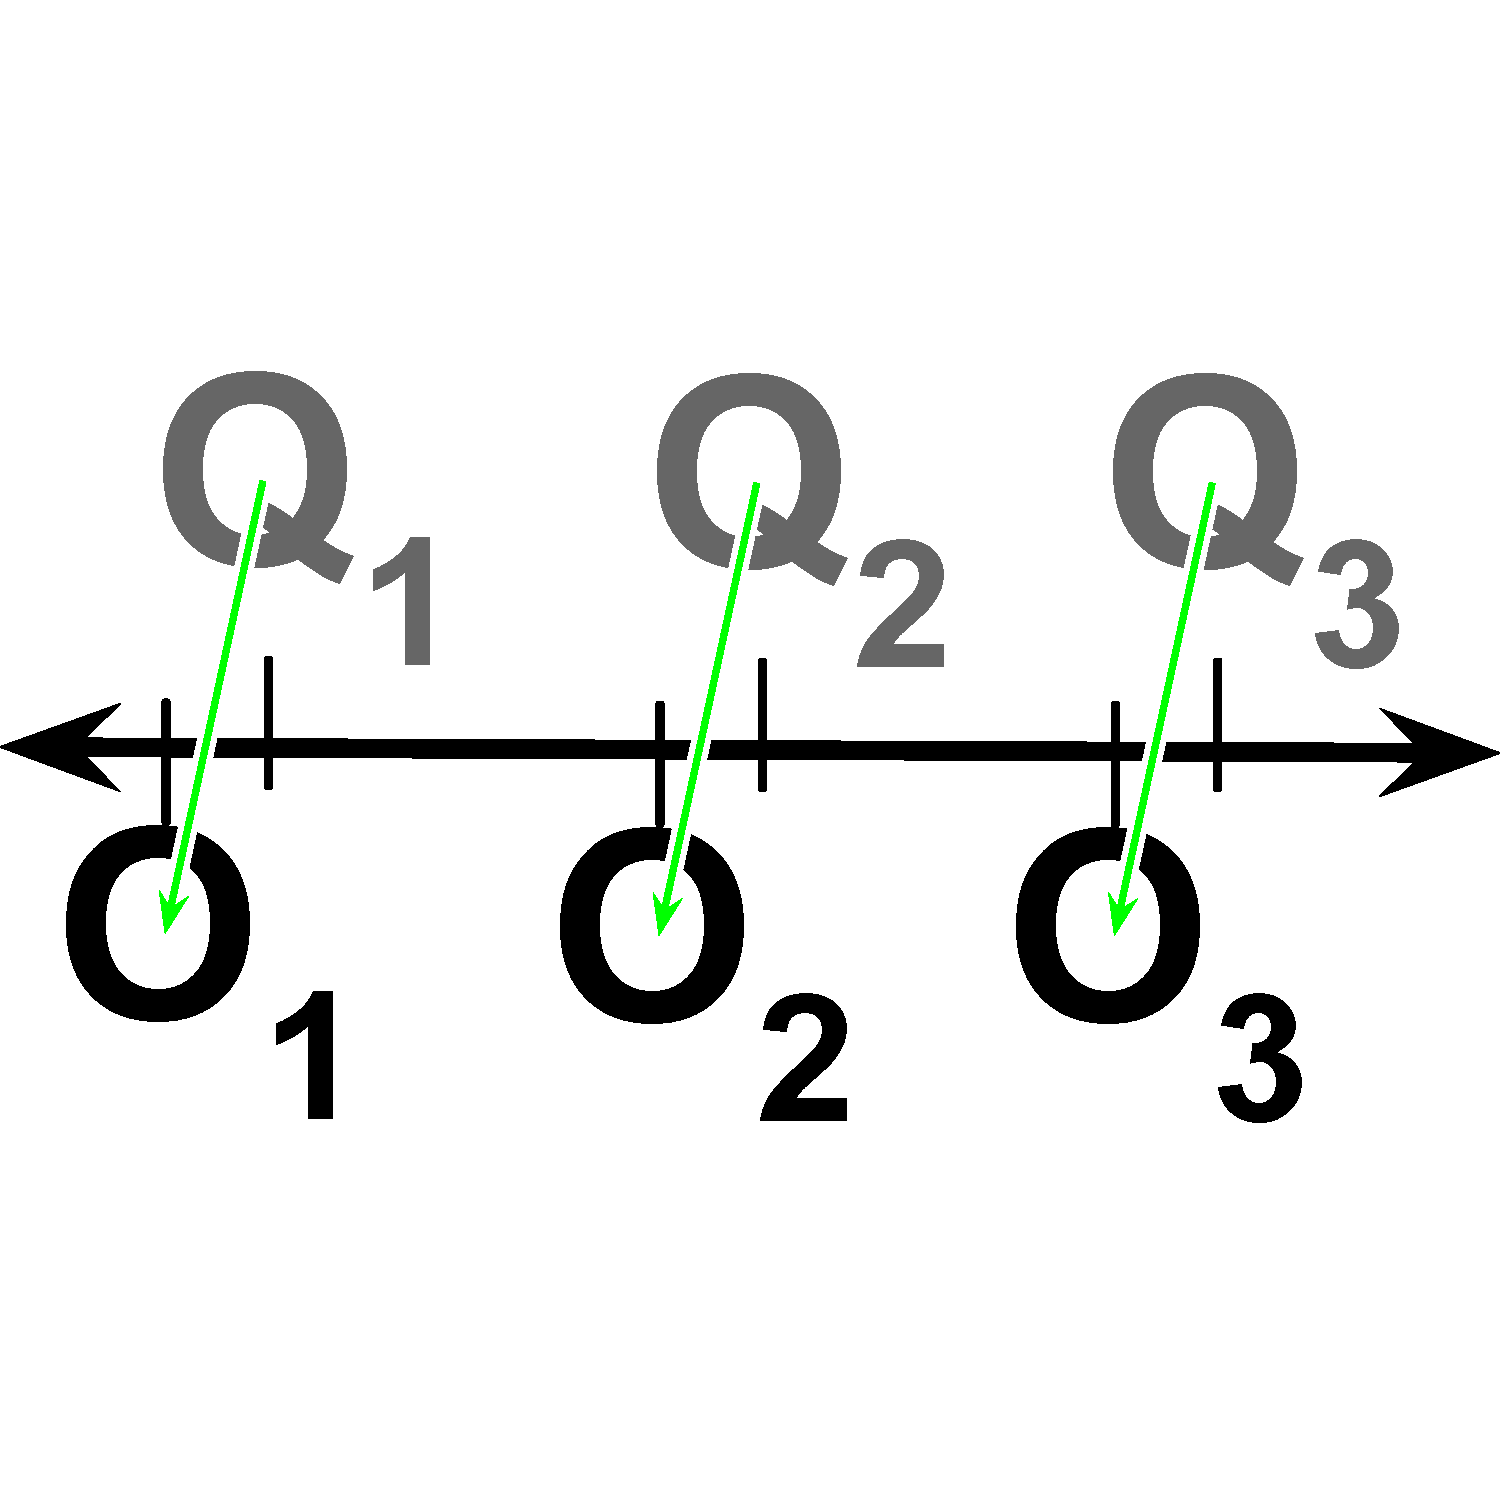
\includegraphics[width=0.33\columnwidth]{{{1d-2d-single-double/1d-single}}}%
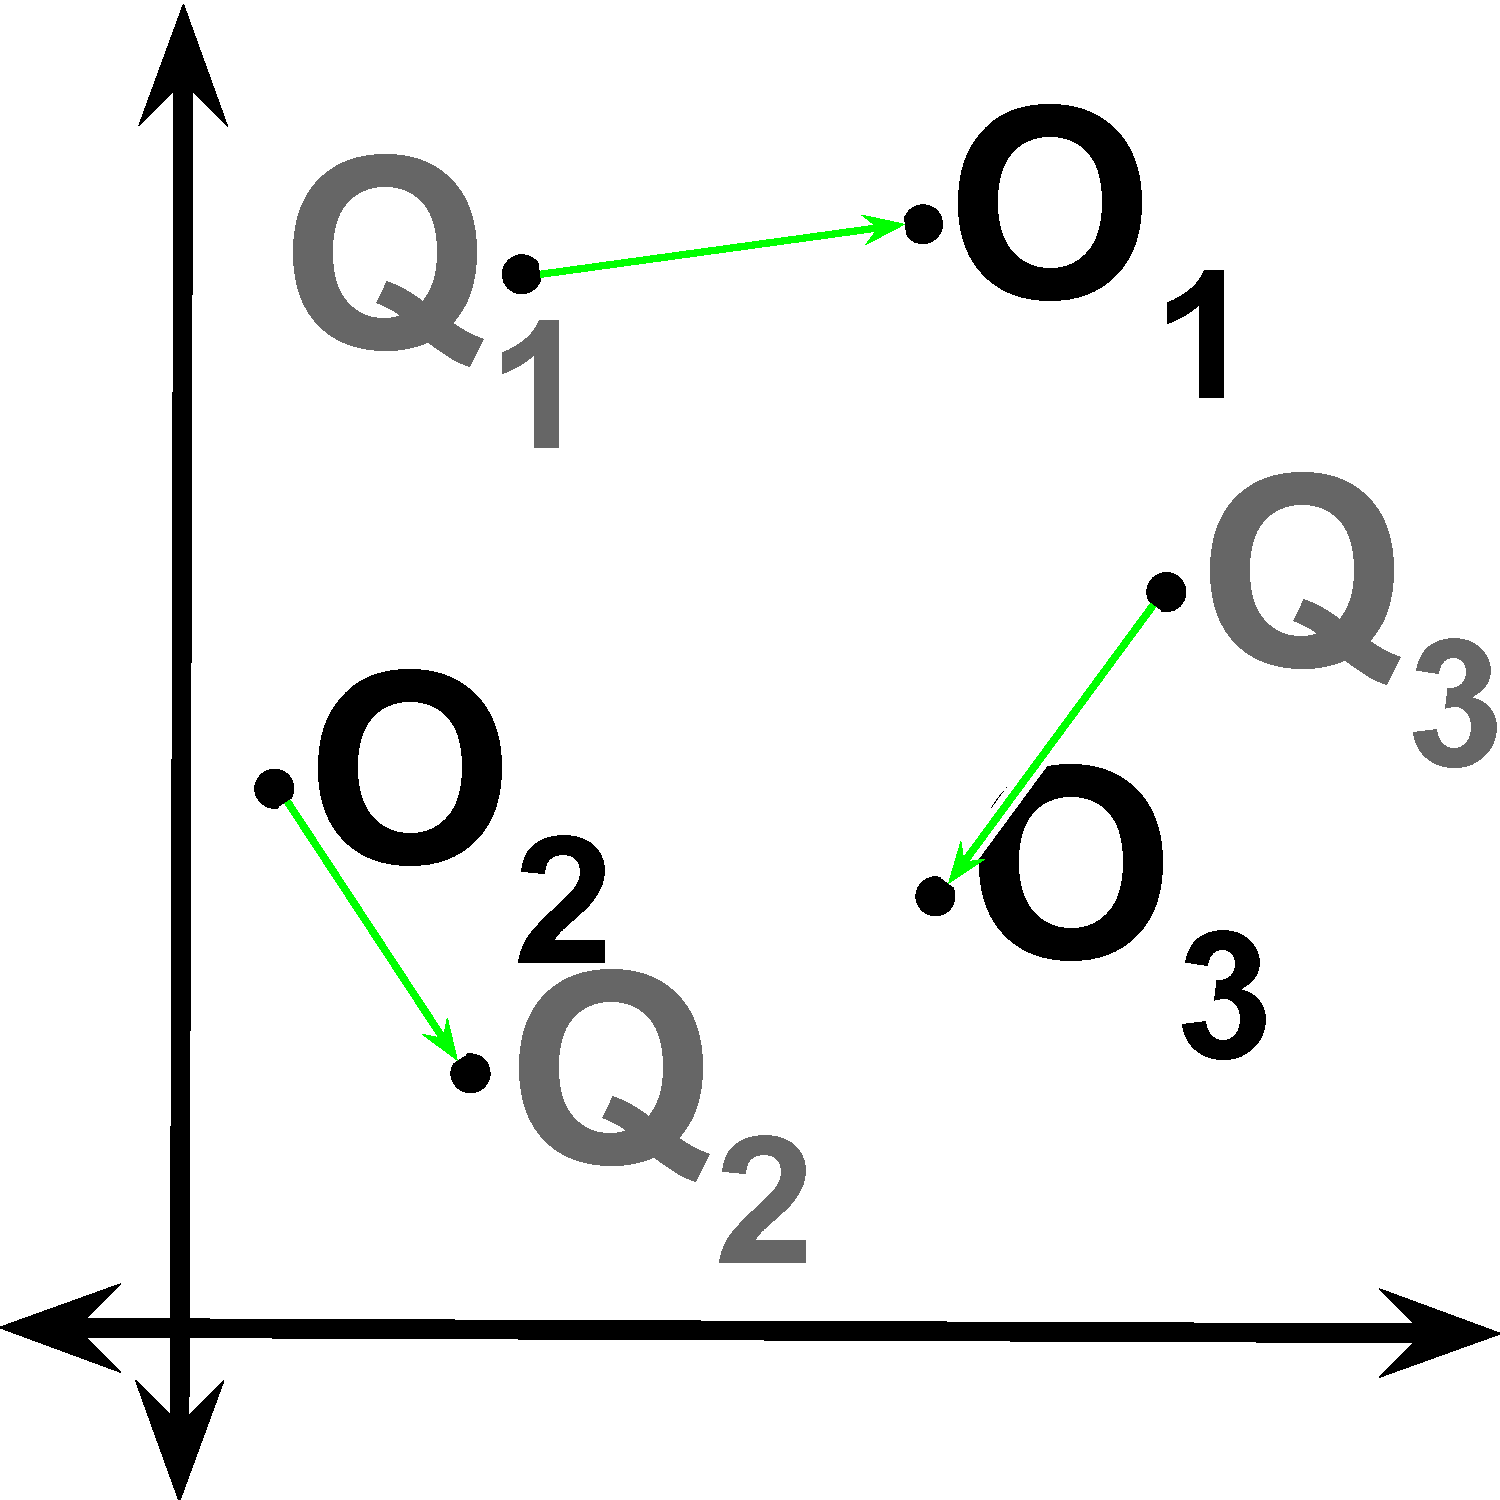
\includegraphics[width=0.33\columnwidth]{{{1d-2d-single-double/2d-single}}}
\caption{
Single-operand matching constraint
}
\label{fig:single}
\end{subfigure}

\begin{subfigure}[b]{\columnwidth}
\centering
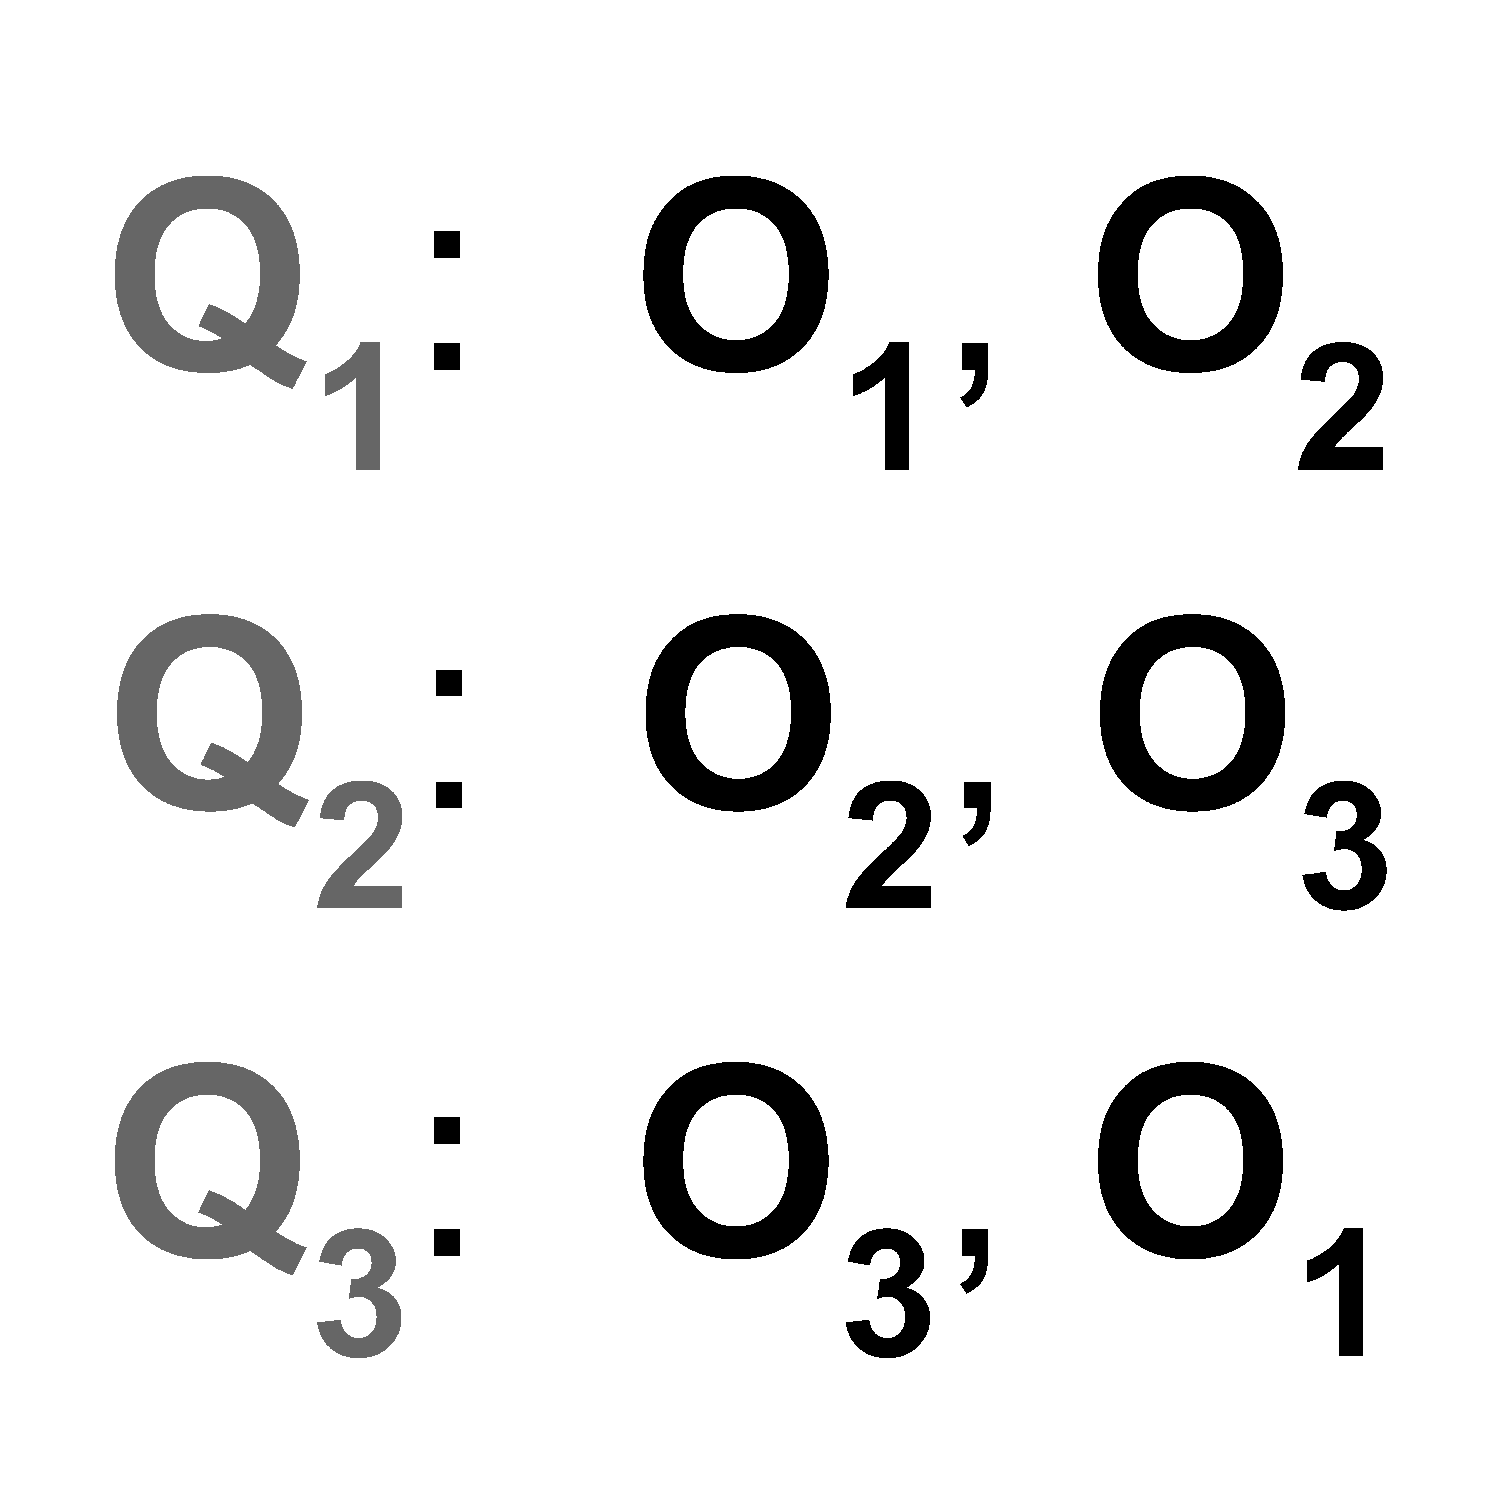
\includegraphics[width=0.33\columnwidth]{{{1d-2d-single-double/double}}}%
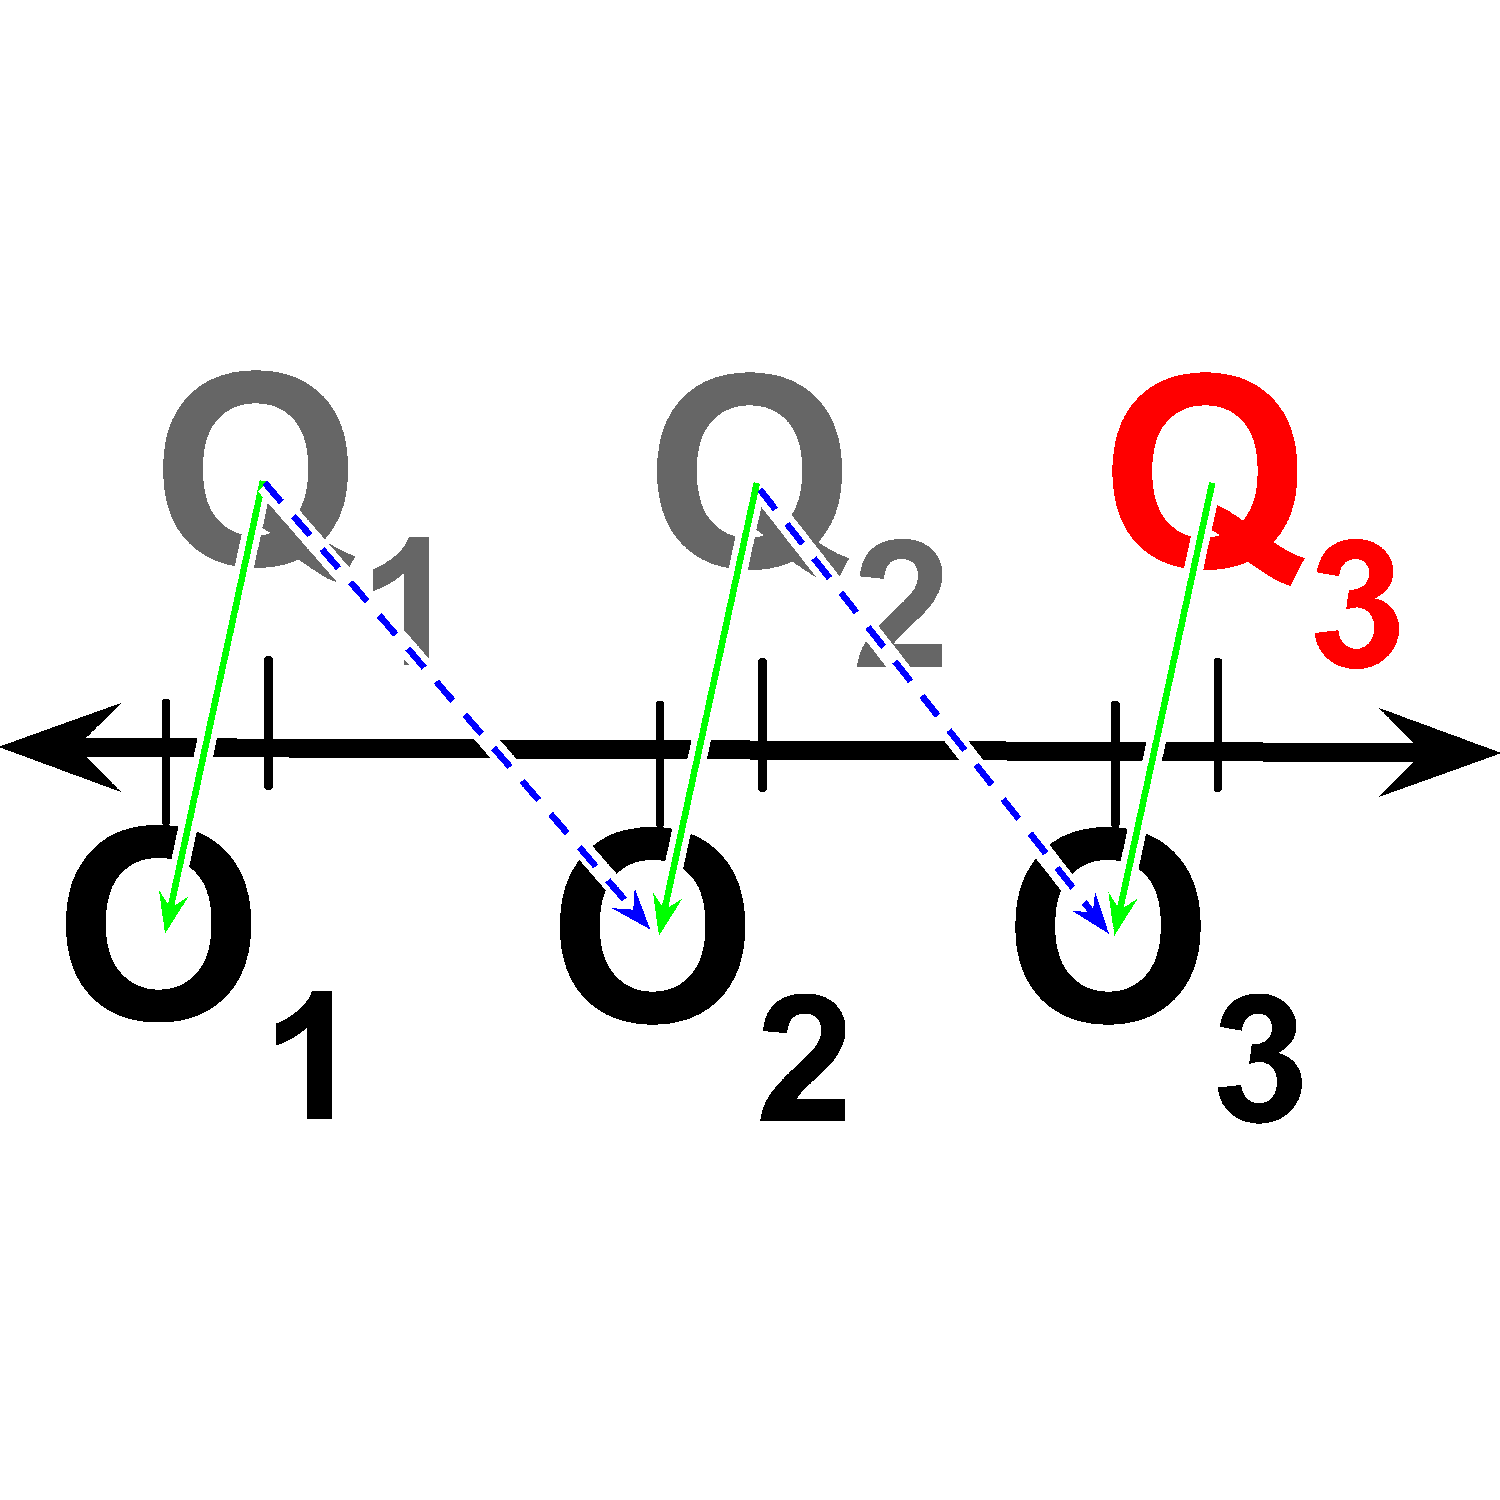
\includegraphics[width=0.33\columnwidth]{{{1d-2d-single-double/1d-double}}}%
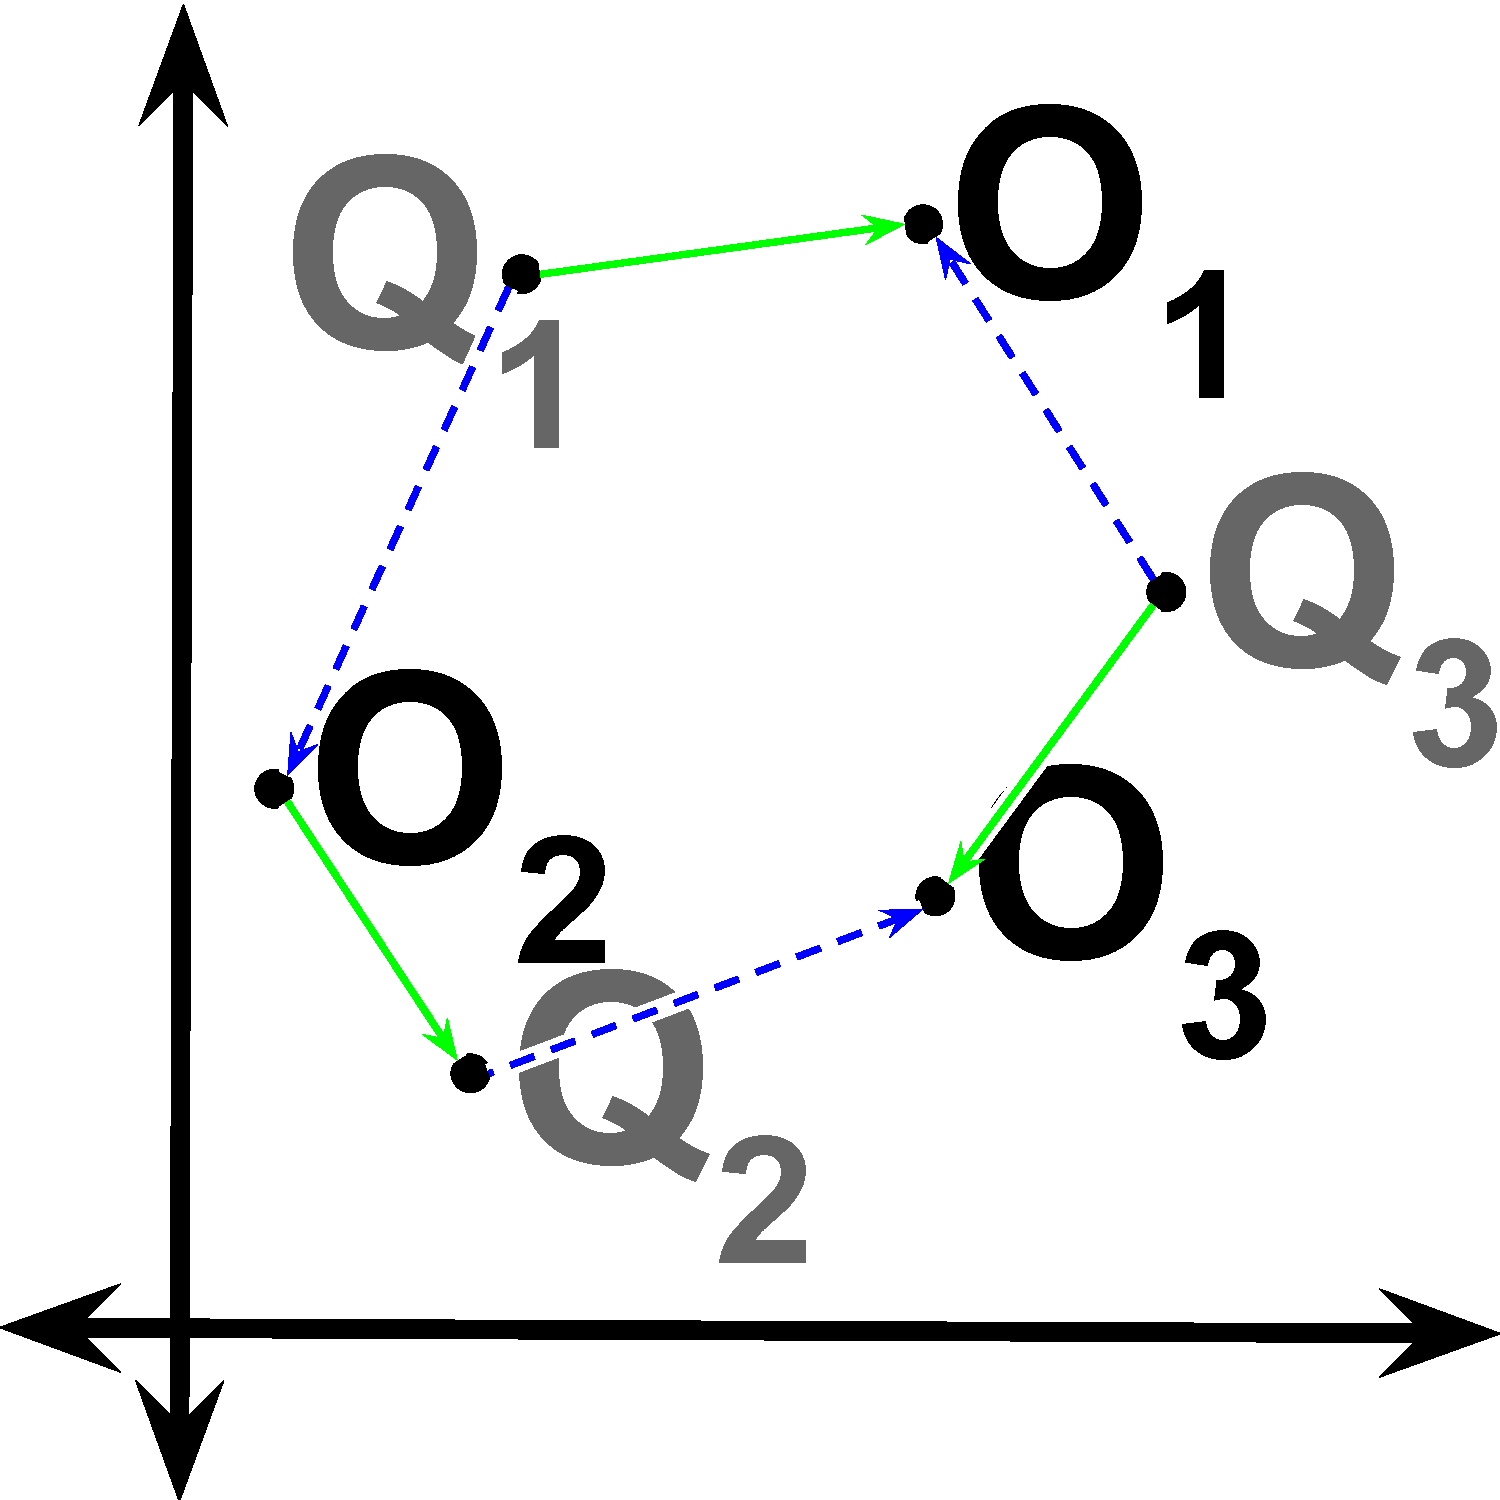
\includegraphics[width=0.33\columnwidth]{{{1d-2d-single-double/2d-double}}}
\caption{
Double-operand matching constraint
}
\label{fig:double}
\end{subfigure}

\caption{
A cartoon depicting the necessity of tag space dimensionality to satisfy multi-operand matching constraints.
}
\label{fig:1d_2d_single_double}

\end{center}
\end{figure}

%Even higher-dimensional metrics are necessary to represent arbitrary longer-match orderings.

%Metrics also differ in their respect for the triangle inequality, that $d(a,c) \leq d(a,b) + d(b,c)$.
%Consider a system in which close matches $d(Q_1, O_2) < t$ and $d(Q_1, O_2) < t$.
%Where also $d(Q_2, O_2) < t$ but $d(Q_2, O_1) > 3t$.
%This is not possible if the triangle inequality holds because we would have $d(Q_2, O_1) < d(Q_2, O_2) + d(Q_1, O_2)+ d(Q_1, O_1) < 3t$.
%Very sad if $3t$ is the similarity threshold for ignoring!
%A similar example can be constructed for a threshold where everything matches (TODO can it?).

%This and also commutativity is also a potentially relevant concern in systems (such as artificial chemistries) where the set of queries and the set of operands are one and the same.

%Tag-matching systems also differ with respect to variation induced under tag mutation.
%A pair of tags matched using the streak metric may both contain neutral sites (e.g., sites not involved in a matching or mismatching streak between the tags) that can mutate freely with no effect on match quality.
%In contrast, a pair of tags matched using hamming or integer metrics contain no neutral sites: every mutation affects match quality.

%Likewise, every individual mutation on a pair of tags matched using the hamming metric has an effect of equal magnitude on match quality.
%However, an individual mutation on a pair of tags matched using the streak metric may have no effect on match quality (e.g., a neutral site), a slight effect on match quality (e.g., on the periphery of a matching or mismatching streak), or a severe effect on match quality (e.g., at the center of a matching or mismatching streak).

The evolutionary consequences of a tag-matching scheme's underlying similarity-defining metric remain unexplored.
Do different tag-matching metrics exhibit different rates of adaptive evolution?
Do tag-matching metrics affect the quality of evolved solutions?
If so, which tag-matching metrics best promote rapid adaptive evolution and high-quality evolved solutions?
And under what circumstances?

In this work, we set out to characterize several tag-matching schemes between bitstring tags that have been proposed in the artificial life and genetic programming literature.

%First, we examine geometric properties of the tag-matching schemes: how do TODO?

%Then, we analyze variational properties of the tag-matching schemes: how do TODO?

%We run a toy target-matching evolutionary experiment to see if these geometric and variational properties have an effect in practice.

%Finally, we throw the different tag-matching schemes into a to test them on diagnostic problems that weren't specifically designed for tag analysis.
